\chapter{Diseño e Implementación} % Main chapter title
\label{Chapter3} % Change X to a consecutive number; for referencing this chapter elsewhere, use \ref{ChapterX}

\definecolor{mygreen}{rgb}{0,0.6,0}
\definecolor{mygray}{rgb}{0.5,0.5,0.5}
\definecolor{mymauve}{rgb}{0.58,0,0.82}

%%%%%%%%%%%%%%%%%%%%%%%%%%%%%%%%%%%%%%%%%%%%%%%%%%%%%%%%%%%%%%%%%%%%%%%%%%%%%
% parámetros para configurar el formato del código en los entornos lstlisting
%%%%%%%%%%%%%%%%%%%%%%%%%%%%%%%%%%%%%%%%%%%%%%%%%%%%%%%%%%%%%%%%%%%%%%%%%%%%%
\lstset{ %
  backgroundcolor=\color{white},   % choose the background color; you must add \usepackage{color} or \usepackage{xcolor}
  basicstyle=\footnotesize,        % the size of the fonts that are used for the code
  breakatwhitespace=false,         % sets if automatic breaks should only happen at whitespace
  breaklines=true,                 % sets automatic line breaking
  captionpos=b,                    % sets the caption-position to bottom
  commentstyle=\color{mygreen},    % comment style
  deletekeywords={...},            % if you want to delete keywords from the given language
  %escapeinside={\%*}{*)},          % if you want to add LaTeX within your code
  %extendedchars=true,              % lets you use non-ASCII characters; for 8-bits encodings only, does not work with UTF-8
  %frame=single,	                % adds a frame around the code
  keepspaces=true,                 % keeps spaces in text, useful for keeping indentation of code (possibly needs columns=flexible)
  keywordstyle=\color{blue},       % keyword style
  language=[ANSI]C,                % the language of the code
  %otherkeywords={*,...},           % if you want to add more keywords to the set
  numbers=left,                    % where to put the line-numbers; possible values are (none, left, right)
  numbersep=5pt,                   % how far the line-numbers are from the code
  numberstyle=\tiny\color{mygray}, % the style that is used for the line-numbers
  rulecolor=\color{black},         % if not set, the frame-color may be changed on line-breaks within not-black text (e.g. comments (green here))
  showspaces=false,                % show spaces everywhere adding particular underscores; it overrides 'showstringspaces'
  showstringspaces=false,          % underline spaces within strings only
  showtabs=false,                  % show tabs within strings adding particular underscores
  stepnumber=1,                    % the step between two line-numbers. If it's 1, each line will be numbered
  stringstyle=\color{mymauve},     % string literal style
  tabsize=2,	                   % sets default tabsize to 2 spaces
  title=\lstname,                  % show the filename of files included with \lstinputlisting; also try caption instead of title
  morecomment=[s]{/*}{*/}
}


En este capítulo se describe el diseño e implementación de los diferentes módulos de firmware del sistema, como así también las diferentes herramientas utilizadas. También se presenta la interfaz para el usuario final y cómo el módulo se integra con los servicios de plataformas en la nube.

\section{Herramientas utilizadas}

En esta sección se detallan las diferentes herramientas y tecnologías utilizadas, tanto a nivel de hardware como de software embebido, justificando la elección en cada caso.

\subsection{Hardware}

La principal elección a nivel de hardware radica en el microcontrolador a utilizar en el módulo. Al momento de realizar la selección, se deben tener en cuenta numerosos factores tales como capacidad de procesamiento, memoria RAM, memoria flash, cantidad de pines GPIO (\emph{General Purpose Input Output}, es decir entradas y salidas de propósito general), interfaces de comunicación, consumo de energía, costos y disponibilidad, entre otros. Lógicamente, algunos factores tendrán más importancia que otros dependiendo de la aplicación.

En el caso del módulo a desarrollar, los requerimientos planteados en la sección \ref{requerimientos} ya imponen restricciones considerables en cuanto a las interfaces de comunicación. Por un lado, debido a la comunicación con la placa de control del electrodoméstico, el microcontrolador debe contar al menos con interfaces de comunicación serie UART, I2C y SPI. Además, para simplificar el desarrollo y lograr un diseño más compacto, se exige que el mismo chip cuente también con las interfaces para la comunicación WiFi y Bluetooth del módulo. Estos requerimientos en cuanto a interfaces reduce considerablemente el abanico de posibilidades.

Por otra parte, al tratarse de un módulo que potencialmente tendría acceso a la misma fuente de alimentación que el electrodoméstico, el consumo de energía no es un factor importante a tener en cuenta al momento de la elección.

Debido a que el trabajo consiste en el desarrollo de un prototipo, es sumamente importante que el microcontrolador cuente con un entorno de desarrollo robusto, tanto a nivel de placas o kits de desarrollo, como a nivel de herramientas de programación. Tener esto cuenta al momento de la elección permite un ahorro sustancial de posterior tiempo de desarrollo. 

Por todo lo expuesto anteriormente, es que se decide utilizar un ESP32 \citep{esp32_overview}, el cual es un microcontrolador de 32 bits desarrollado por la compañía Espressif Systems y que cuenta con todas las interfaces de comunicación requeridas integradas en el mismo chip, tal como puede verse en la tabla \ref{tab:esp32_interfaces}.

\begin{table}[h]
	\centering
	\caption{Interfaces de comunicación disponibles en un microcontrolador ESP32.}
	\begin{tabular}{c c}    
		\toprule
		\textbf{Interfaz de comunicación}	& \textbf{Cantidad}	\\
		\midrule
		WiFi								& 1					\\
		BLE									& 1					\\
		UART 								& 3					\\		
		SPI	 								& 4					\\
		I2C	 								& 2					\\
		\bottomrule
		\hline
	\end{tabular}
	\label{tab:esp32_interfaces}
\end{table}

Además el microcontrolador ESP32 cuenta con un excelente entorno de programación, numerosas placas de desarrollo, una documentación oficial de gran calidad y una comunidad muy activa.

En la figura \ref{fig:nodemcu_esp32} se puede observar la placa de desarrollo para ESP32 utilizada para el desarrollo de este trabajo, llamada NodeMCU \citep{esp32_nodemcu}. Esta placa se eligió principalmente por su gran disponibilidad en el mercado local.

\begin{figure}[h]
\centering
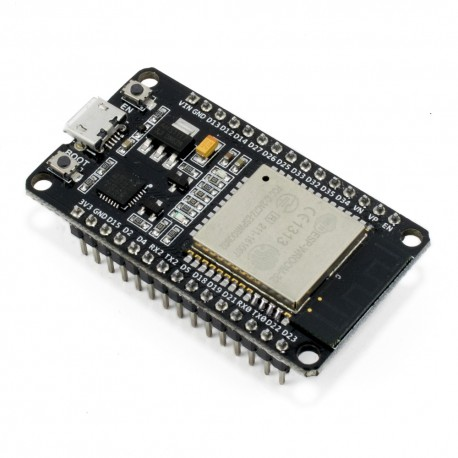
\includegraphics[scale=0.4]{./Figures/nodemcu_esp32.jpg}
\caption[Placa de desarrollo para ESP32 NodeMCU.]{Placa de desarrollo para ESP32 NodeMCU.\footnotemark}
\label{fig:nodemcu_esp32}
\end{figure}

\footnotetext{Imagen extraída de \url{https://naylampmechatronics.com/espressif-esp/384-placa-de-desarrollo-para-esp32-nodemcu-32.html}.}

Cabe mencionar que la placa de desarrollo no utiliza directamente el microcontrolador ESP32, sino que usa el módulo ESP32-WROOM \citep{esp32_wroom}, el cual es un chip que posee en su interior un ESP32, pero contiene además una memoria flash de 4MB conectada a este y una antena de PCB integrada para la conectividad WiFi y Bluetooth, entre algunas otras funcionalidades.

\subsection{Software embebido}

A nivel de software embebido, la principal decisión pasa por determinar si es necesario utilizar un sistema operativo de tiempo real (RTOS por sus siglas en inglés correspondientes a \emph{Real Time Operating System}).

Si bien el módulo no requiere cumplir con restricciones de tiempo real, un RTOS ofrece otras atractivas características que justifican su uso. Entre estas características, la de mayor utilidad es la capacidad de gestionar la ejecución de múltiples tareas. Además ofrecen otras herramientas que resultan de gran utilidad como temporizadores o colas para comunicar tareas entre sí. También permiten integrar con mayor facilidad librerías que implementen funcionalidades complejas como los protocolos TCP/IP.

Por ello es que, dada la complejidad del sistema a implementar, en el que se requieren múltiples tareas ejecutándose y comunicándose entre sí, sumado a la necesidad de recurrir a una implementación del \emph{stack} TCP/IP, se decide utilizar un sistema operativo de tiempo real.

A su vez existen numerosas alternativas al momento de determinar qué RTOS utilizar. Sin embargo, el microcontrolador ESP32 ya cuenta con todo un entorno de desarrollo denominado ESP-IDF (\emph{Espressif IoT Development Framework}), el cual es una versión de FreeRTOS \citep{freertos} modificada para trabajar de manera óptima con este microcontrolador. Por ello se decide utilizar este \emph{framework} para el desarrollo del firmware y por lo tanto FreeRTOS como sistema operativo de tiempo real.

\subsection{Plataforma en la nube}
\label{plataforma_nube}

Para que el fabricante del electrodoméstico pueda almacenar, analizar y visualizar la información de sus diferentes electrodomésticos conectados, es sumamente conveniente recurrir a una plataforma de servicios en la nube. Estas plataformas se ocupan de gestionar toda la infraestructura necesaria asociada a la administración de dispositivos, autenticación, almacenamiento, análisis de datos, y mucho más.

Existen diferentes alternativas de plataformas que se pueden usar para lograr este objetivo, siendo las más conocidas las ofrecidos por Google (Google Cloud Platform \citep{google_cloud_platform}), Amazon (Amazon Web Services \citep{aws}) y Microsoft (Microsoft Azure \citep{microsoft_azure}). En los tres casos tienen servicios similares orientados específicamente a la Internet de las Cosas: Google Cloud IoT Core, AWS IoT y Azure IoT, respectivamente. Un gran atractivo de las tres plataformas, es que ofrecen un saldo inicial considerable que permite utilizar sus servicios sin necesidad de incurrir en gastos. Además muchos servicios pueden ser utilizados sin costo indefinidamente, con ciertas restricciones en cuanto a recursos disponibles y con un consumo que debe mantenerse por debajo de ciertos valores. Esto permite probar las tres plataformas y atravesar toda la etapa de desarrollo y prototipado sin que ello sea un costo adicional. 

Tras llevar a cabo un exhaustivo análisis para determinar cuál de las tres plataformas utilizar, y debido a que las tres plataformas cuentan con características muy similares, se decidió utilizar Google Cloud Platform principalmente por las siguientes causas:

\begin{itemize}
	\item La autenticación de los dispositivos es más sencilla y utiliza mecanismos estándar. 
	\item La curva de aprendizaje inicial es menos pronunciada, lo que permite agilizar el desarrollo.
	\item Los dispositivos se pueden comunicar tanto por HTTP/S como por MQTT.
\end{itemize}

Al utilizar Google Cloud Platform, se hace también un uso exhaustivo de Google Cloud IoT Core, el cual es un servicio completamente administrado que permite conectar, administrar y transferir datos con rapidez y seguridad desde millones de dispositivos (o desde tan sólo unos pocos) en todo el mundo \citep{iot_core}. Además, Google Cloud IoT Core puede combinarse con otros servicios de la plataforma, para así tener a disposición una solución completa para recopilar, procesar, analizar y visualizar datos de IoT en tiempo real.

\section{Firmware}

Para implementar las funcionalidades explicadas en la sección \ref{funcionamiento_general}, fue necesario desarrollar a nivel de firmware diferentes módulos que interactúan entre sí, como puede verse en el diagrama de la figura \ref{fig:fw_diagram}. En la arquitectura planteada, cada uno de los módulos del diagrama se corresponde con una tarea que se ejecuta en el sistema operativo de tiempo real. 

\begin{figure}[h]
\centering
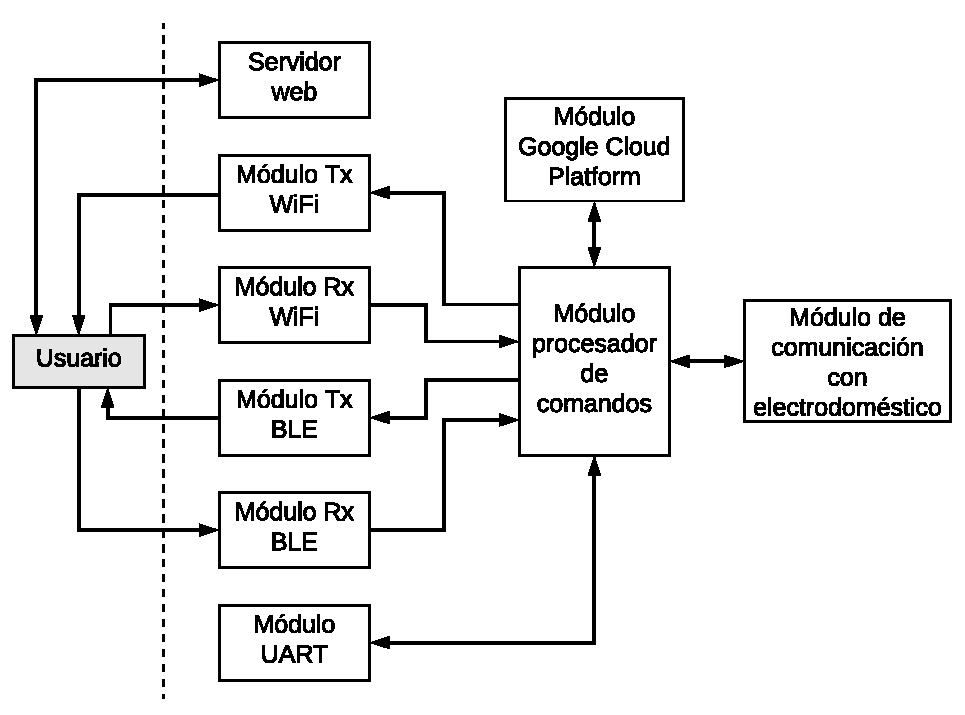
\includegraphics[width=\textwidth]{./Figures/firmware_diagram.pdf}
\caption{Diagrama de bloques de los módulos de firmware implementados.}
\label{fig:fw_diagram}
\end{figure}

De esta forma se tiene un módulo central (módulo procesador de comandos en el diagrama) que se encarga de recibir y procesar todos los comandos, y de generar todas las respuestas necesarias, abstrayéndose del origen o destino de los mismos. Es decir que si el usuario del electrodoméstico manda un determinado comando por WiFi o Bluetooth, el módulo procesador de comandos es quien lo recibe en ambos casos, y luego se encarga de enviar la respuesta al módulo correspondiente (WiFi o Bluetooth según sea el caso). Además, este módulo es el único que interactúa con el módulo encargado de la comunicación con el electrodoméstico, por lo que toda comunicación con este debe pasar necesariamente a través del procesador de comandos. Esta centralización permite tener un gran control acerca de cómo ocurre la interacción entre los módulos y las prioridades al momento de atender más de una consulta. La sincronización y el pasaje de datos entre las diferentes tareas de cada módulo y el procesador de comandos se lleva a cabo mediante colas o \emph{queues} \citep{freertos_queues}.

Por otra parte, se tienen los módulos encargados tanto de recibir los comandos enviados por el usuario y enviarlos al módulo procesador de comandos, como así también de recibir las respuestas para enviarlas nuevamente al usuario. Estos son los módulos Tx (transmisor, es decir el que envía la respuesta al usuario) y Rx (receptor, es decir el que recibe el comando del usuario), tanto WiFi como Bluetooth. En secciones posteriores se profundiza más sobre la implementación específica de estos módulos, pero a grandes rasgos se ocupan de manejar toda la interacción necesaria con el hardware y los \emph{drivers} asociados a la comunicación WiFi/Bluetooth. También se encargan de detectar el comando/respuesta recibido y enviarlo a donde corresponda. 

Cabe mencionar que en el caso de los módulos WiFi, se cuenta con tres implementaciones diferentes, una para cada uno de los protocolos de aplicación soportados: HTTP, HTTPS y MQTT. Si bien en los tres casos se reutiliza en su totalidad todo lo asociado a la interacción con el hardware, la forma de enviar y recibir información difiere considerablemente. Además, solamente uno de los tres protocolos se puede soportar en simultáneo, debido principalmente a limitaciones de memoria RAM, que impide asignar el \emph{stack} suficiente para todas las tareas a la vez. Por ello es que mediante banderas del compilador (\emph{compiler flags}), se especifica qué protocolo usará la imagen de firmware generada.

En la figura \ref{fig:fw_diagram} también se observa un módulo UART, que a diferencia de los otros módulos de transmisión y recepción, no interactúa con el usuario. Esto se debe a que es una tarea que se incluyó sólo con fines de \emph{debug}, ya que permite enviar y recibir los mismos comandos que a través de las interfaces inalámbricas, pero de una forma mucho más simple utilizando una de las interfaces UART del microcontrolador.

Como se mencionó en la sección \ref{plataforma_nube}, para que el fabricante del electrodoméstico pueda analizar y visualizar la información de sus electrodomésticos conectados, se utiliza Google Cloud Platform. El módulo desarrollado envía periódicamente información acerca de su estado, para que luego esta información sea almacenada, analizada y visualizada a lo largo del tiempo. De esto precisamente se encarga el módulo Google Cloud Platform. Cada vez que la tarea requiere obtener el estado del electrodoméstico, lo hace a través del procesador de comandos, enviando un comando de manera muy similar a como lo haría el usuario.

Otro de los módulos involucrados en la comunicación WiFi es el del servidor web. Esta tarea se encuentra corriendo permanentemente de fondo, y permite que el usuario, conectándose a una red WiFi local generada por el propio microcontrolador (que actúa también como punto de acceso), ingrese a una página web que permite configurar las credenciales de la red WiFi del hogar a la cual el módulo se debe conectar.

Finalmente, se tiene el módulo de comunicación con el electrodoméstico. Esta tarea se encuentra la mayor parte del tiempo bloqueada, esperando que el procesador de comandos se comunique con ella, con el objetivo de disparar alguna acción en el electrodoméstico. Una vez que lo hace, la tarea se comunica con el artefacto mediante la interfaz serie correspondiente. Dado que el electrodoméstico se emula mediante otro microcontrolador que cuenta con una interfaz I2C, ésta es la que se emplea para la comunicación serie.


\subsection{Comunicación WiFi}

Para lograr una comunicación con una página web externa en Internet desde el microcontrolador, es necesario contar con implementaciones de todas las capas del modelo TCP/IP. Para ello, se utilizaron en su mayor parte librerías ya existentes optimizadas para sistemas embebidos, tal como puede observarse en la tabla \ref{tab:implementacion_capas}.


\begin{table}[h]
	\centering
	\caption{Capas del modelo TCP/IP con sus correspondientes protocolos e implementaciones en el microcontrolador.}
	\begin{tabular}{l l l}    
		\toprule
		\textbf{Capa del modelo TCP/IP}	& \textbf{Protocolo}	& \textbf{Implementación}	\\
		\midrule
		Aplicación			& HTTP/HTTPS/MQTT		& ESP-IDF					\\
		Seguridad			& TLS					& mbed TLS					\\
		Transporte			& TCP					& lwIP						\\
		Internet			& IP					& lwIP						\\
		Acceso a la red 	& WiFi					& ESP-IDF					\\
		\bottomrule
		\hline
	\end{tabular}
	\label{tab:implementacion_capas}
\end{table}

Para manejar la comunicación a más bajo nivel mediante WiFi, se recurre al \emph{driver} que forma parte del \emph{framework} ESP-IDF desarrollado por el propio fabricante del microcontrolador. Este \emph{driver} expone una API con ciertas funciones que el programador puede llamar para interactuar con la interfaz WiFi del chip. También se debe definir un \emph{event handler} (manejador de eventos), es decir una función que el \emph{driver} WiFi llama cada vez que debe notificar un nuevo evento que haya ocurrido. En la figura \ref{fig:wifi_driver} se puede apreciar esta interacción entre el \emph{driver} y el programa principal.

\begin{figure}[h]
\centering
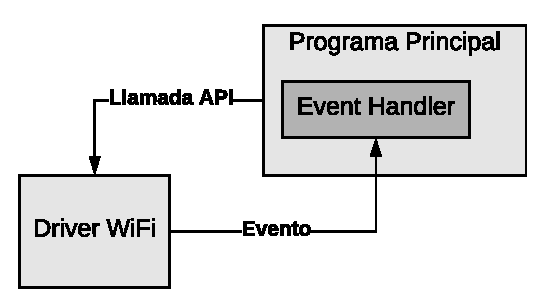
\includegraphics[scale=1.0]{./Figures/wifi_driver.pdf}
\caption{Interacción entre el driver WiFi y el programa principal.}
\label{fig:wifi_driver}
\end{figure}

El \emph{driver} WiFi permite utilizar la interfaz en tres modos diferentes:
\begin{itemize}
	\item Modo estación (\emph{station mode}) o modo cliente WiFi, en el que el microcontrolador se conecta a un punto de acceso.
	\item Modo punto de acceso (\emph{AP mode}), en el que el microcontrolador actúa como un punto de acceso al que otros clientes se conectan.
	\item Modo combinado (\emph{combined AP-STA mode}), en el que el microcontrolador se comporta como punto de acceso y a la vez como una estación que se conecta a otro punto de acceso.
\end{itemize}

En este trabajo se utiliza el modo combinado, ya que se requiere que el chip funcione como estación (para conectarse a la red WiFi del hogar que le da salida a Internet) y como punto de acceso (para que el usuario pueda acceder al servidor web que corre en el microcontrolador).

Con respecto al \emph{event handler}, los eventos de interés que gestiona son los siguientes:

\begin{itemize}
	\item STA\_START: se dispara luego de que el driver se ha inicializado como estación. En este punto es posible conectarse a una red en particular.
	\item STA\_GOT\_IP: se dispara cuando se logra una conexión exitosa a una red y se obtiene una dirección IP.
	\item STA\_DISCONNECTED: se genera cuando se produce una desconexión de la red.
	\item AP\_START: se dispara luego de que el driver se ha inicializado como punto de acceso. En este punto se puede comenzar a ejecutar el servidor web.
	\item AP\_STACONNECTED: se produce cuando una estación se conecta al punto de acceso.
	\item AP\_STADISCONNECTED: se genera cuando una estación se desconecta del punto de acceso.
\end{itemize}

Muchas tareas necesitan tener conocimiento de los eventos que gestiona el \emph{event handler}, principalmente requieren conocer cuándo el módulo ha logrado conectarse a la red deseada. Para lograr esta sincronización se utilizan \emph{event groups} \citep{event_groups}, cuyos bits se programan en el \emph{event handler} del \emph{driver} WiFi. Por ejemplo, cuando se establece una conexión exitosa a una red, el bit 0 del \emph{event group} se pone en 1 y así se disparan de manera sincronizada aquellas tareas que estaban esperando que se establezca dicha conexión.

Continuando con las próximas capas del modelo, para las de Transporte/Internet, se hace uso de los protocolos TCP/IP. Para ello se utiliza la librería lwIP \citep{lwip}, que es una implementación de código abierto de los protocolos TCP/IP diseñada para sistemas embebidos, ya que busca minimizar al máximo la utilización de recursos.

El protocolo TCP/IP no proporciona ningún tipo de seguridad para la red en la que se los utiliza. Sin embargo, es posible agregar una capa adicional por encima de la de transporte, que permita establecer una comunicación segura, encriptada y autenticada a lo largo de una red no segura. Esta seguridad adicional para la capa de transporte se denomina \emph{Transport Layer Security} (TLS) \citep{tls} y para su implementación se recurre a la librería mbed TLS \citep{mbed_tls}.

Finalmente, para la capa de aplicación se utilizan tres protocolos diferentes: HTTP, HTTPS y MQTT. En el caso de HTTPS y MQTT la comunicación es segura ya que se utiliza también TLS, mientrás que para el protocolo HTTP la información no se transmite de manera segura y podría ser interceptada en el camino.

Como ya se mencionó anteriormente, los tres protocolos no son soportados en forma simultánea, sino que en tiempo de compilación se decide cuál de ellos se va a usar en la imagen generada.

En el caso de los protocolos HTTP y HTTPS, si bien el \emph{framework} ESP-IDF ya cuenta con implementaciones de clientes, se decide llevar a cabo una implementación propia a los fines de profundizar los conocimientos en la temática. Para ello, en el cliente HTTP se utiliza la librería lwIP para crear los \emph{sockets} necesarios y realizar las escrituras y lecturas necesarias, creando métodos para enviar una HTTP \emph{request} y recibir una HTTP \emph{response}. El caso del cliente HTTPS es más complejo, y se utiliza la libreria mbed TLS para crear todas las estructuras necesarias para la transacción segura, y luego también se definen métodos para enviar \emph{requests} y recibir \emph{responses}, incluyendo el proceso del \emph{handshake} TLS \citep{tls_handshake}.

Una vez implementados los clientes HTTP y HTTPS, se los utiliza en los respectivos módulos de transmisión y recepción de comandos por WiFi. Las tareas implementadas son relativamente sencillas y muy similares para ambos protocolos, diferenciándose principalmente en las funciones que llaman para enviar y recibir información. En la figura \ref{fig:http_tx_task_diagram} se puede apreciar un diagrama de flujo de la tarea de transmisión por WiFi usando HTTP/HTTPS. Cabe mencionar que el que envía datos nuevos a la cola de la tarea es el procesador de comandos, cuando desea devolver una respuesta al usuario.

\begin{figure}[h]
\centering
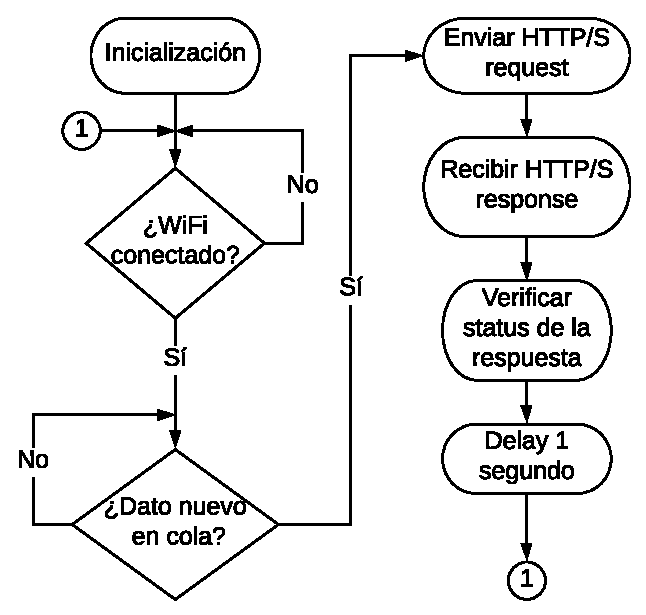
\includegraphics[scale=0.75]{./Figures/http_tx_task_diagram.pdf}
\caption{Diagrama de flujo para las tareas de transmisión por HTTP/HTTPS.}
\label{fig:http_tx_task_diagram}
\end{figure}

Por otra parte, en la figura \ref{fig:http_rx_task_diagram} se observa un diagrama de flujo de las tareas de recepción de comandos empleando HTTP/HTTPS. El funcionamiento básico de esta tarea consiste en consultar periódicamente si el usuario ha enviado un nuevo comando, y en caso afirmativo reenviarlo al procesador de comandos.

\begin{figure}[h]
\centering
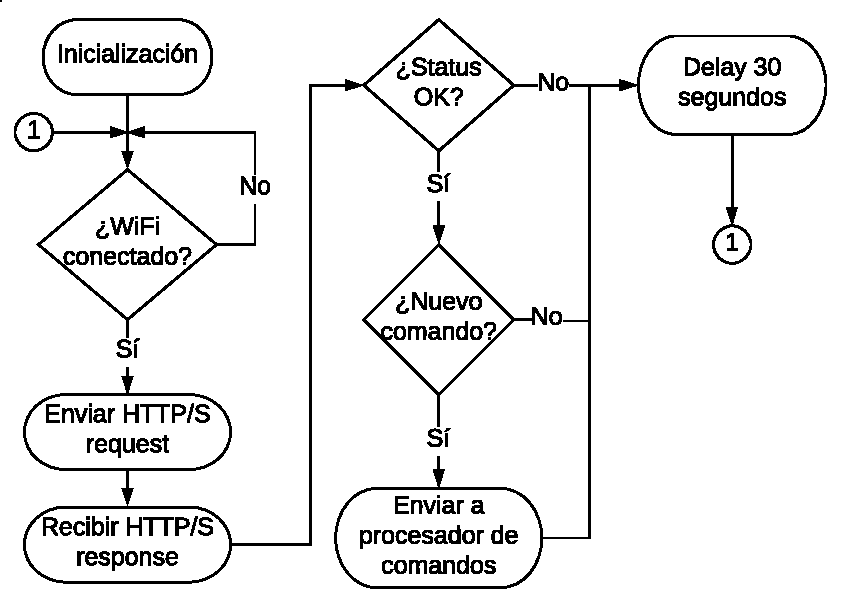
\includegraphics[scale=0.75]{./Figures/http_rx_task_diagram.pdf}
\caption{Diagrama de flujo para las tareas de recepción por HTTP/HTTPS.}
\label{fig:http_rx_task_diagram}
\end{figure}


Finalmente, para el caso de los módulos WiFi con protocolo MQTT, se decide utilizar directamente las implementaciones del protocolo que ya forman parte del \emph{framework} ESP-IDF, debido a que una implementación propia resultaría demasiado compleja y escapa al alcance de este trabajo. El funcionamiento general de las tareas es análogo al de las versiones con HTTP/HTTPS, con la diferencia de que ahora se utiliza MQTT para publicar las respuestas hacia el usuario en un \emph{topic} determinado, y recibir comandos desde otro \emph{topic} al cual el microcontrolador se encuentra subscripto. El protocolo MQTT se utiliza sobre TLS, por lo tanto todos los intercambios de información ocurren de manera segura.

De manera similar al \emph{driver} WiFi, se implementa un \emph{event handler} que gestiona los siguientes eventos asociados al protocolo MQTT:

\begin{itemize}
	\item MQTT\_EVENT\_CONNECTED: se dispara cuando se logra una conexión exitosa con el \emph{broker} MQTT.
	\item MQTT\_EVENT\_DISCONNECTED: se genera ante una desconexión del \emph{broker}.
	\item MQTT\_EVENT\_SUBSCRIBED/UNSUBSCRIBED/PUBLISHED: se produce cada vez que un cliente MQTT se suscribe, elimina la suscripción o publica datos en un \emph{topic} determinado.
	\item MQTT\_EVENT\_DATA: se genera cada vez que un \emph{topic}, al que algún cliente se encuentra suscripto, recibe información nueva y la envía al cliente MQTT.
\end{itemize} 

%\subsection{Arquitectura MQTT}


\subsection{Comunicación BLE}

Un dispositivo BLE puede actuar como \emph{peripheral} (periférico o servidor) o como \emph{central} (principal o cliente), y en el caso de este trabajo el microcontrolador actúa como un \emph{peripheral}. El servidor anuncia continuamente su presencia, enviando paquetes para que otros dispositivos detecten su presencia. Por su parte, el dispositivo \emph{central}, que en este caso sería la aplicación en el celular del usuario del electrodoméstico, realiza un escaneo en busca de dispositivos cercanos. Una vez que encuentra el \emph{peripheral} deseado, establece una conexión y le realiza diferentes peticiones.

De manera similar al caso del WiFi, se cuenta con un \emph{driver} que gestiona la interfaz Bluetooth y se comunica con el programa principal mediante eventos. En este caso se deben definir varios \emph{event handlers} para gestionar diferentes facetas de la comunicación. Para entender el funcionamiento de la comunicación BLE implementada es necesario comprender también algunos conceptos asociados al propio protocolo. 

Por un lado se tiene el concepto de GAP (\emph{Generic Access Profile}), que controla las conexiones y el \emph{advertising}, es decir cómo el servidor anuncia su presencia transmitiendo paquetes periódicamente. Mediante las estructuras de datos y funciones que el \emph{framework} expone, se especifican diferentes parámetros como el \emph{advertising interval} (cada cuánto el dispositivo anuncia su presencia) o el nombre del dispositivo, entre muchos otros. Además se tiene un \emph{event handler} para los eventos asociados al GAP, entre los que se destacan dos en particular:

\begin{itemize}
	\item GAP\_BLE\_ADV\_DATA\_SET\_COMPLETE\_EVT: se dispara cuando los parámetros de \emph{advertising} se encuentran configurados, y por lo tanto se lo utiliza para iniciar el proceso de \emph{advertising}. Es decir que cuando este evento se detecta, el dispositivo comienza a anunciar su presencia.
	\item GAP\_BLE\_ADV\_START\_COMPLETE\_EVT: este evento indica que el proceso de \emph{advertising} terminó su inicialización, y se lo puede utilizar para determinar si dicha inicialización tuvo éxito u ocurrió alguna falla. 
\end{itemize}

En cuanto a la forma de transmitir datos, el intercambio de información entre dos dispositivos BLE se realiza mediante los denominados atributos genéricos o GATT (\emph{Generic Attributes}), los cuales son estructuras de datos jerárquicas que constituyen la base del protocolo. Esta jerarquía puede observarse en la figura 

En cuanto a la forma de transmitir datos, el intercambio de información entre dos dispositivos BLE se realiza mediante los denominados atributos genéricos o GATT (\emph{Generic Attributes}), los cuales son estructuras de datos jerárquicas que constituyen la base del protocolo. Esta jerarquía puede observarse en la figura \ref{fig:gatt} y está constituida por varias partes:

\begin{itemize}
	\item Perfil (\emph{profile}): es la jerarquía de mayor nivel y está formada por uno o más servicios.
	\item Servicio (\emph{service}): es un conjunto de diferentes informaciones (como lecturas de un sensor), y contiene por lo menos una característica. Existen numerosos servicios predefinidos por el Bluetooth Special Interest Group (SIG), como presión sanguínea o ritmo cardíaco, y además se pueden crear servicios personalizados en caso de que el uso no esté contemplado en esa lista predefinida, como es el caso de este trabajo.
	\item Característica (\emph{characteristic}): es donde se encuentran los datos propiamente dichos. Posee varios campos, entre los que se destacan el de \emph{value}, con el valor en sí, y el de \emph{properties}, que describe cómo se puede interactuar con el valor.
\end{itemize}

\begin{figure}[h]
\centering
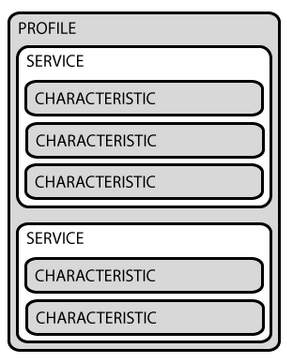
\includegraphics[scale=0.5]{./Figures/gatt.png}
\caption[Jerarquía de la estructura GATT.]{Jerarquía de la estructura GATT.\footnotemark}
\label{fig:gatt}
\end{figure}

\footnotetext{Imagen extraída de \url{https://learn.adafruit.com/introduction-to-bluetooth-low-energy/gatt}.}

Un cliente puede llevar a cabo diferentes operaciones sobre una característica de un \emph{peripheral}, incluyendo operaciones de lectura y escritura. Esto justamente es lo que se utiliza para enviar comandos por BLE (se escribe una característica en particular) y para recibir respuestas (se lee una característica).

Se implementa también un \emph{event handler} para los eventos asociados a GATT, entre los cuales se destacan los siguientes:

\begin{itemize}
	\item GATTS\_REG\_EVT: es el primer evento que se dispara al iniciar el servidor BLE. Se lo utiliza para configurar los parámetros de \emph{advertising} (lo cual dispara luego el correspondiente evento en el \emph{event handler} de GAP) y para crear el servicio que usa la aplicación.
	\item GATTS\_CREATE\_EVT: es el próximo evento en dispararse luego de que el servicio se crea exitosamente. Se lo usa para iniciar el servicio y para agregarle las características que luego se usan para enviar comandos y recibir respuestas.
	\item GATTS\_CONNECT\_EVT/GATTS\_DISCONNECT\_EVT: se dispara cada vez que un cliente se conecta/desconecta del \emph{peripheral}.
	\item GATTS\_WRITE\_EVT: se produce cuando el dispositivo cliente desea realizar una operación de escritura sobre una característica, es decir cuando el usuario desea mandar un comando al electrodoméstico. En este punto se lee lo que el usuario escribió en la característica y se lo envía al procesador de comandos.
	\item GATTS\_READ\_EVT: se produce cuando el cliente desea realizar una operación de lectura sobre una característica, es decir cuando el usuario desea recibir una respuesta del electrodoméstico. Para ello se escribe en la característica correspondiente el valor que se recibe desde el procesador de comandos.
\end{itemize}


\subsection{Procesamiento de comandos}

La tarea que se encarga de procesamiento de comandos se encuentra en todo momento que algún módulo escriba en la cola correspondiente. Se utiliza una única cola a la que todos los módulos envían datos, a través de una estructura que incluye no solamente el comando propiamente dicho, sino también un identificador del módulo que escribió en la cola, tal como puede verse en el algoritmo 3.1.

\begin{lstlisting}[label=rx_command_struct:vControl,caption=Pseudocódigo del lazo principal de control.]
/*------------------------------------------------------------------
|  Struct: rx_command_t
| ------------------------------------------------------------------
|  Description: represents a received command.
|
|  Members:
|       rx_id   - module that sent the command
|       command - command received
*-------------------------------------------------------------------*/
typedef struct {
    rx_module_t     rx_id;
    command_type_t  command; 
}   rx_command_t;
\end{lstlisting}

Cuando se necesita enviar una respuesta, se utiliza ese \emph{rx\_id} para determinar el módulo adecuado y por lo tanto en qué cola se debe escribir la respuesta.

El tipo de dato \emph{command\_type\_t} define los diferentes comandos disponibles, y es fácilmente extensible con nuevos valores. Existen dos grupos de comandos:

\begin{itemize}
	\item Comandos dirigidos al módulo: no se comunican con el electrodoméstico, sino que actúan solamente sobre el módulo de conectividad.
	\begin{itemize}
		\item CMD\_WIFI: se utiliza para cambiar el estado de la conexión WiFi (si está apagada la enciende, si está encendida la apaga). Debido a que el WiFi y el BLE no pueden estar funcionando en simultáneo, en caso de que este último se encuentre encendido, se lo desactiva antes de iniciar la conexión WiFi.
		\item CMD\_BLE: análogo a CMD\_WIFI, pero aplicado a Bluetooth Low Energy.
		\item CMD\_ECHO: comando utilizado para \emph{debug}, simplemente le devuelve a la misma interfaz los mismos datos que envió.
	\end{itemize}
	\item Comandos dirigidos al electrodoméstico: son una serie de comandos genéricos a modo de ejemplo, los cuales se envían por I2C al microcontrolador que emula al electrodoméstico.
	\begin{itemize}
		\item CMD\_SLAVE\_START\_A/CMD\_SLAVE\_START\_B: inicia en el electrodoméstico un determinado proceso.
		\item CMD\_SLAVE\_PAUSE: pausa el proceso actual.
		\item CMD\_SLAVE\_CONTINUE: reanuda un proceso pausado.
		\item CMD\_SLAVE\_RESET: reinicia el electrodoméstico.
		\item CMD\_SLAVE\_STATUS: se lo emplea para preguntar por el estado actual del electrodoméstico.
	\end{itemize}
\end{itemize}

Para el microcontrolador que emula el comportamiento del electrodoméstico, el cual también es un ESP32, se desarrolló un firmware simplificado con una tarea principal que consiste en una máquina de estados, la cual representa los diferentes estados del electrodoméstico. Los comandos que recibe por su interfaz I2C pueden modificar esta máquina de estados, reflejando así que un determinado proceso inicia o termina. Además, cada vez que recibe un comando desde el módulo principal, le devuelve al mismo una señal de \emph{acknowledge}, la cual es verificada por la tarea de procesamiento de comandos cada vez que se produce una comunicación con el electrodoméstico.

\section{Integración con Google Cloud Platform}

Como se mencionó en la sección \ref{plataforma_nube}, para proporcionarle información al fabricante acerca del estado del electrodoméstico se utiliza Google Cloud Platform. Esta implementación tiene dos facetas: por un lado la tarea a nivel de firmware que permite que el microcontrolador se comunique con Google Cloud, y por el otro toda la infraestructura y los servicios utilizados en Google Cloud.

Se utilizan diferentes servicios de Google Cloud Platform, y el principal de ellos es Cloud IoT Core. Este servicio cuenta con dos componentes principales:

\begin{itemize}
	\item \emph{Device manager} (administrador de dispositivos): permite registrar y administrar dispositivos, y ofrece también un mecanismo para autenticarlos cuando se conectan. El módulo desarrollado se registra aquí como dispositivo.
	\item \emph{Protocol bridge} (puente de protocolos): permite acceder a Google Cloud de manera segura mediante protocolos MQTT y HTTP.
\end{itemize}

El servicio de Cloud IoT Core interactúa con varios otros servicios de Google Cloud para armar un flujo de análisis completo, como puede observarse en la figura \ref{fig:google_cloud_diagram}.

\begin{figure}[h]
\centering
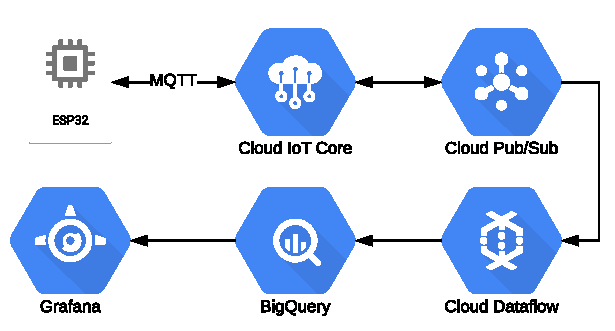
\includegraphics[width=\textwidth]{./Figures/google_cloud_diagram.pdf}
\caption{Arquitectura utilizada en Google Cloud Platform.}
\label{fig:google_cloud_diagram}
\end{figure}

El servicio más importante con el que interactúa es Cloud Pub/Sub, ya que es el servicio en el cual se publican todos los datos recibidos por el \emph{protocol bridge}. De hecho cada dispositivo en Cloud IoT Core tiene asociado al menos un \emph{topic} en Cloud Pub/Sub, y es en ese \emph{topic} donde el microcontrolador realiza la publicación de los datos que desee.

En este punto ya se tiene almacenada toda la información cruda enviada por el electrodoméstico, y los bloques restantes se encargan de mostrar gráficamente esa información utilizando Grafana, que es una herramienta que permite la visualización de datos provenientes de distintas fuentes. En este caso se utiliza como fuente Big Query, una base de datos altamente eficiente y escalable ofrecida por Google Cloud. Para que los datos de los \emph{topics} se transfieran y almacenen automáticamente a la base de datos, se utiliza Cloud Dataflow. Finalmente se utiliza la propia infraestructura de Google Cloud para levantar la aplicación de Grafana, pudiendo así finalmente visualizar los datos enviados por el dispositivo.

Por otro lado, a nivel de firmware se cuenta con una tarea dedicada exclusivamente a enviar periódicamente a Google Cloud información acerca del estado actual del electrodoméstico. Esta transmisión se lleva a cabo solamente utilizando el protocolo MQTT, es decir que no hay soporte para HTTP/HTTPS. 

El principal desafío para enviar la información está en las autenticaciones necesarias para que esto sea posible. 

Por un lado, debido a que la transmisión es segura (utiliza TLS por debajo) es necesario utilizar los certificados de Google Cloud Platform al momento de configurar el cliente MQTT. Esto no difiere del procedimiento realizado para las tareas de MQTT que interactúan con el usuario.

También es necesario autenticar el dispositivo en particular, es decir el microcontrolador debe demostrar que cuando se comunica con Google Cloud, es el dispositivo que dice ser y no otro haciéndose pasar por él \citep{device_security}. Para ello es necesario generar claves, asociar dichas claves a cada dispositivo en Cloud IoT Core, y luego almacenar la clave también en el firmware. La figura \ref{fig:device_key} ilustra este proceso.

\begin{figure}[h]
\centering
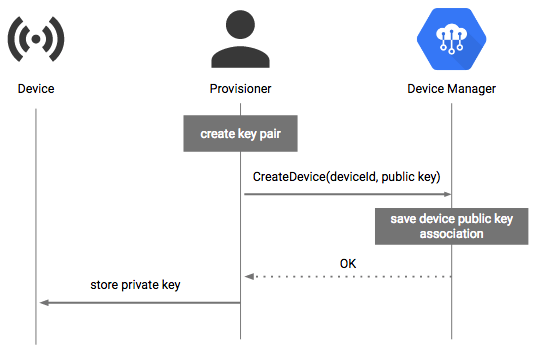
\includegraphics[scale=0.55]{./Figures/device_key.png}
\caption[Proceso de generación de claves para el servicio de Cloud IoT Core.]{Proceso de generación de claves para el servicio de Cloud IoT Core.\footnotemark}
\label{fig:device_key}
\end{figure}

\footnotetext{Imagen extraída de \url{https://cloud.google.com/iot/docs/concepts/device-securityprovisioning_credentials}.}


Luego el firmware debe utilizar la clave que tiene almacenada para generar un JSON Web Token (JWT) \citep{jwt} y enviarlo al momento de conectarse por MQTT, como se observa en la figura \ref{fig:device_key}.

\begin{figure}[h]
\centering
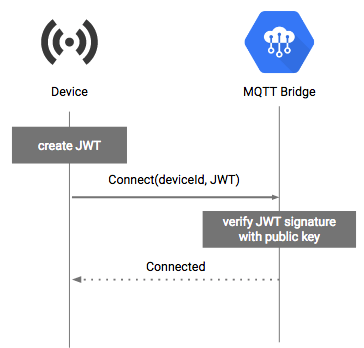
\includegraphics[scale=0.7]{./Figures/device_jwt.png}
\caption[Autenticación del dispositivo utilizando un JWT.]{Autenticación del dispositivo utilizando un JWT.\footnotemark}
\label{fig:device_jwt}
\end{figure}

\footnotetext{Imagen extraída de \url{https://cloud.google.com/iot/docs/concepts/device-securityprovisioning_credentials}.}

